\documentclass{article}

% Language setting
% Replace `english' with e.g. `spanish' to change the document language
\usepackage[portuguese]{babel}

% Set page size and margins
% Replace `letterpaper' with `a4paper' for UK/EU standard size
\usepackage[letterpaper,top=2cm,bottom=2cm,left=3cm,right=3cm,marginparwidth=1.75cm]{geometry}
\usepackage{listings}
\usepackage{xcolor}
\usepackage{longtable}
\usepackage{geometry}

\definecolor{bqBackground}{RGB}{250, 250, 250}
\definecolor{bqKeywords}{RGB}{66, 139, 202}
\definecolor{bqStrings}{RGB}{194, 56, 14}
\definecolor{bqIdentifiers}{RGB}{97, 97, 97}
\definecolor{bqComments}{RGB}{150, 150, 150}
\definecolor{bqFunction}{RGB}{97, 97, 97}
\definecolor{bqType}{RGB}{0, 0, 255}

\lstset{
    backgroundcolor=\color{bqBackground},   
    basicstyle=\ttfamily\footnotesize,
    keywordstyle=\color{bqKeywords}\bfseries,
    stringstyle=\color{bqStrings},
    identifierstyle=\color{bqIdentifiers},
    commentstyle=\color{bqComments}\itshape,
    morekeywords={SELECT, FROM, AS},  % BigQuery keywords
    moredelim=[s][\color{bqStrings}]{`}{`},  % for backticks
    showstringspaces=false,
    numbers=left,
    numberstyle=\tiny\color{gray},
    numbersep=5pt,
    tabsize=2,
    captionpos=b,
    breaklines=true,
    frame=single,
    rulecolor=\color{gray}
}


% Useful packages
\usepackage{amsmath}
\usepackage{graphicx}
\usepackage[colorlinks=true, allcolors=blue]{hyperref}

\title{Desafio CIVITAS}
\author{Filipe S P Prates \\ filipespprates@gmail.com}

\begin{document}
\maketitle

\section{Introdução}

Este artigo apresenta os métodos e resultados obtidos em resposta ao Desafio Civitas, demonstrando minhas habilidades em análise de dados.
Utilizarei os dados da tabela `rj-cetrio.desafio.readings\_2024\_06`, que contém leituras de radares de trânsito do município do Rio de Janeiro.

Para mais informações, visite o repositório do \href{https://github.com/prefeitura-rio/emd-desafio-civitas}{desafio CIVITAS no github}.

\section{Objetivo}
O objetivo do desafio é realizar uma análise exploratória dos dados, identificar inconsistências, além de identificar placas de veículos que foram possivelmente clonadas, usando as informações disponíveis.

\section{Análise Exploratória dos Dados}

\subsection{Esquema dos Dados}

Os dados fornecidos representam instâncias de capturas de radares de trânsito. Cada entrada na tabela contém informações referentes à uma captura: um veículo em uma posição em um momento do tempo. As colunas disponíveis estão descritas na Tabela \ref{tab:description}.

\begin{table}
\centering
\begin{tabular}{|l|l|l|}
\hline
Coluna           & Tipo       & Descrição                                 \\\hline
datahora         & TIMESTAMP  & Data e hora da detecção do radar          \\\hline
datahora\_captura & TIMESTAMP  & Data e hora do recebimento dos dados      \\\hline
placa            & BYTES      & Placa do veículo capturado                \\\hline
empresa          & BYTES      & Empresa do radar                          \\\hline
tipoveiculo      & BYTES      & Tipo do veículo                           \\\hline
velocidade       & INTEGER    & Velocidade do veículo                     \\\hline
camera\_numero    & BYTES      & Número identificador do radar             \\\hline
camera\_latitude  & FLOAT      & Latitude do radar                         \\\hline
camera\_longitude & FLOAT      & Longitude do radar                        \\\hline
\end{tabular}
\caption{\label{tab:description}Descrição das colunas da tabela.}
\end{table}

\subsection{Informações Gerais dos Dados}
O dataset disponibilizado contém informações sobre 36.358.536 capturas de radares. Realizadas entre "2024-06-06 00:00:00 UTC" (5 de Junho de 2024, 9 horas da noite no Rio de Janeiro), até "2024-06-13 14:31:56 UTC" (13 de Junho de 2024, 11 horas e 31 minutos da manhã no Rio de Janeiro).


\subsection{Coluna Categóricas}
Das colunas da tabela, \textit{placa}, \textit{empresa}, \textit{tipoveiculo} e \textit{camera\_numero} são colunas categóricas, ou seja, possuem uma série de valores pré-fixados que podem receber. Nesta subseção analisamos para tais colunas, quantos valores distintos para cada categoria existem, e como estão os dados distribuídos entre eles.


São representados no dataset 7.984.610 \textit{placas} diferentes, com um total de 36.358.536 capturas, resultando em uma média de aproximadamente 4.55 capturas para cada placa.

Apenas 3 \textit{empresas} são responsáveis por todos os registros de capturas no Dataset (Figura  \ref{fig:registrosPorEmpresa}).

O sistema classifica os veículos refistrados em 4 \textit{tipoveiculo}s diferentes, observando as velocidades médias de cada tipo de veículo, podemos propôr hipóteses de qual \textit{tipoveiculo} refere a qual tipo de veículo real (Figura \ref{fig:tipoVeiculoAvgSpeed}).

Utilizaremos à frente á fim de otimização de cáculos o fato de todos os 36 milhões de registros estarem agrupados geograficamente em apenas 1421 radares fixos.

\begin{figure}
    \centering
    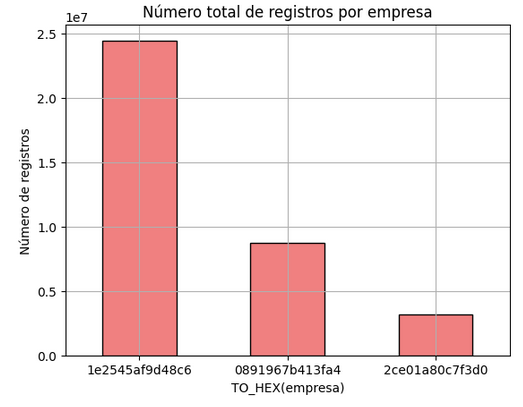
\includegraphics[width=0.5\linewidth]{registrosPorEmpresa.png}
    \caption{Número de registros por empresa responsável. A empresa 1e2545af9d48c6, com 24 milhões de registros, tem responsabilidade sobre aproximadamente 67\% do Dataset. Essa distribuição é similar ao número de câmeras por empresa.}
    \label{fig:registrosPorEmpresa}
\end{figure}

\begin{figure}
    \centering
    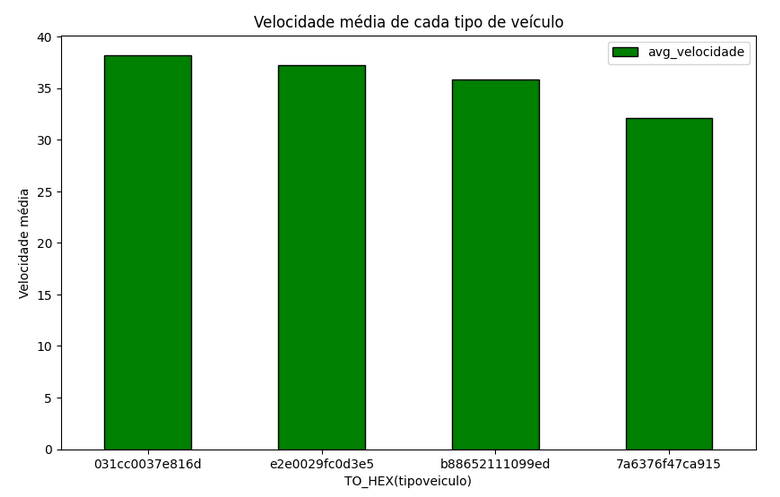
\includegraphics[width=0.75\linewidth]{tipoVeiculoAvgSpeed3.png}
    \caption{Velocidades médias de cada tipo de veículo. Podemos observar uma variação entre as velocidade médias dependendo do tipo de veículo. De 32.1 km/h para veículos do tipo 7a6376f47ca915, até 38.2km/h para veículos do tipo 031cc0037e816d. Os dados são consistentes em 7a6376f47ca915 representar veículos de carga como caminhões, enquanto 031cc0037e816d e e2e0029fc0d3e5 representam motos e veículos de passeio. }
    \label{fig:tipoVeiculoAvgSpeed}
\end{figure}


\begin{lstlisting}[language=SQL,caption={Query SQL para contar quantidade de valores distintos para as colunas categóricas do dataset},label={lst:sqlquery}]
SELECT COUNT(DISTINCT placa) AS unique_placas
FROM `rj-cetrio.desafio.readings_2024_06`;

SELECT COUNT(DISTINCT empresa) AS unique_empresas
FROM `rj-cetrio.desafio.readings_2024_06`;

SELECT COUNT(DISTINCT tipoveiculo) AS unique_tipoveiculo
FROM `rj-cetrio.desafio.readings_2024_06`;

SELECT COUNT(DISTINCT camera_numero) AS unique_radares
FROM `rj-cetrio.desafio.readings_2024_06`;
\end{lstlisting}

\begin{table}
\centering
\begin{tabular}{|l|l|}
\hline
Coluna         & Número de valores distintos \\\hline
placa          & 7984610 \\\hline
empresa        & 3       \\\hline
tipoveiculo  & 4       \\\hline
camera\_numero & 1421    \\\hline
\end{tabular}
\caption{\label{tab:categorics}Valores distintos de cada coluna categóricas.}
\end{table}

\subsubsection{Número de registros por cada câmera de radar}

Observamos na Figura \ref{fig:freqCameraNumeroTop30} que a câmera de radar identificada por f6b6eff6c3c578 é a que mais registrou veículos no Dataset, com aproximadamente o dobro de registros da segunda com mais registros. Tal câmera, infelizmente, é uma das que indica \textit{camera\_latitude} e \textit{camera\_longitude} sempre 0 como posteriormente iremos investigar, logo não é possível testar a hipótese que essa câmera deve estar na principal via da cidade.

\begin{figure}
    \centering
    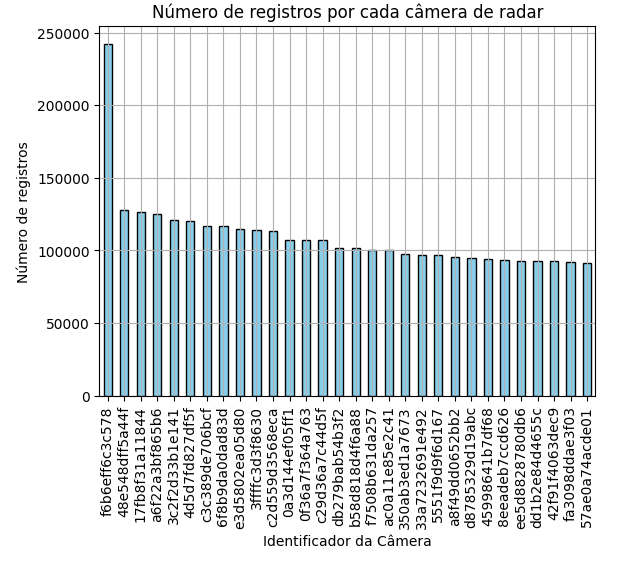
\includegraphics[width=0.75\linewidth]{freqCameraNumeroTop30.png}
    \caption{As 30 câmeras de radares com mais registros, e seu número de registros, do Município do Rio de Janeiro.}
    \label{fig:freqCameraNumeroTop30}
\end{figure}

Ao analisar todas as câmeras exceto a f6b6eff6c3c578, percebemos uma distribuição similar à uma exponencial. Onde poucas câmeras são responsáveis pela maioria dos registros, e muitas câmeras possuem poucos registros. Isto é consistente com uma rede complexa de ruas, onde algumas vias são muito utilizadas, e outras, mais capilares, pouco utilizadas. Figura \ref{fig:lineCameraNumeroInverted}.

\begin{figure}
    \centering
    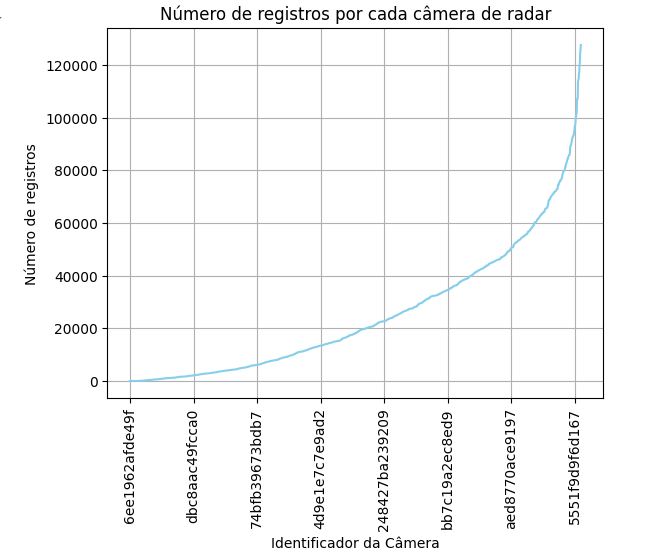
\includegraphics[width=0.75\linewidth]{lineCameraNumeroInverted.png}
    \caption{Número de registros por câmera de radares, ordenados da câmera com menos registros (6ee1962afde49f, 457ee59cde6d92 e bb059f56ccf5e3, com um registro cada) até a câmera com mais registros (48e548dff5a44f, já que foi excluida a outlier camera\_numero f6b6eff6c3c578). Observamos um comportamento de regime exponencial - onde câmeras localizadas em vias com grande fluxo de carros geram uma parte muito maior dos registros se comparadas à radares em ruas menos frequentadas.}
    \label{fig:lineCameraNumeroInverted}
\end{figure}
\subsection{Histograma de Velocidades}

As velocidades dos veículos registradas no dataset foram consideradas consistentes com o Município do Rio de Janeiro, vide Figura \ref{fig:histVelocidades}.

\begin{figure}
    \centering
    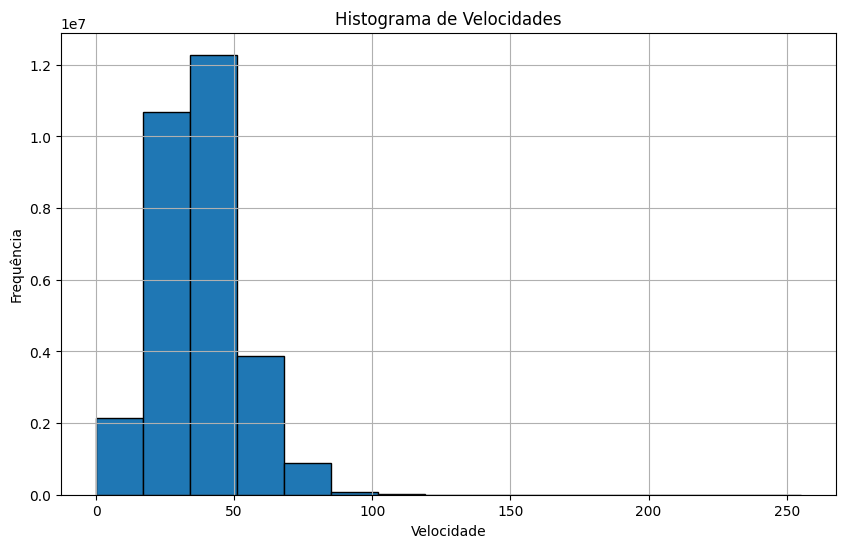
\includegraphics[width=0.75\linewidth]{histVelocidades.png}
    \caption{Histograma com as frequencias que as diferentes velocidades foram registradas pelo radares do Rio de Janeiro. Observamos uma distribuição normal em volta da média de aproximadamente 35km/h, consistente com ruas urbanas, com alguns outliers de até 255 km/h. Tais valores são altos, porém, devido à sua pequena frequência, considerados ainda consistentes com uma metrópole com vias expressas e milhões de habitantes.}
    \label{fig:histVelocidades}
\end{figure}

Investigando mais a fundo as velocidades acima de 200km/h, percebemos que por via de regra se concentram em poucas câmeras de radar, pricipalmente em vias expressas como por exemplo o \textit{camera\_numero} 2633b189184a46, que contém 390 casos de registros de velocidade superior à 200km, localizado na Av. das Américas próximo do número 4069. Nos casos de radares em ruas secundárias poderíamos remover os dados como inconsistentes, porém em casos em vias expressas, assumimos como dados reais.

\begin{lstlisting}[language=SQL,caption={Query SQL para identificar quais as câmeras de radares mais capturam veículos em velocidades superiores à 200km/h, a fim de investigar suas latitudes e longitudes, e assim determinar se o registro é potencialmente válido, ou não.},label={lst:sqlquery10}]
SELECT TO_HEX(camera_numero), camera\_latitude, camera\_longitude, count(*)
FROM `rj-cetrio.desafio.readings_2024_06`
WHERE velocidade > 200
group by camera_numero
\end{lstlisting}

\subsection{Inconsistência nos dados de Latitude e Longitude}

Algumas das câmeras de radares registram latitudes e longitudes inconsistentes. Por exemplo, no caso da \textit{camera\_numero} CKF78vkvCg==, todos os seus registros indicam \textit{camera\_latitude} e \textit{camera\_longitude} 0. Ao todo \textbf{259 casos} de câmeras que não registram latitudes e longitudes consistentes com o território do Município do Rio de Janeiro. Neste artigo tais registros serão desconsiderados, porém com acesso ao endereço de tais câmeras, seria possível corrigir os valores e então acrescentar mais registros para análise.

\begin{lstlisting}[language=SQL,caption={Query SQL para identificar se existem casos inconsistentes onde câmeras registram valores de latitude e longitude fora do território do Município do Rio de Janeiro. Existem 259 casos de câmeras com problemas sistemáticos neste quesito.},label={lst:sqlquery2}]
SELECT 
    distinct camera_numero, 
FROM 
    `rj-cetrio.desafio.readings_2024_06`
WHERE 
    camera_latitude >= -22.8
  OR camera_latitude <= -23.0
  OR camera_longitude <= -43.8
  OR camera_longitude >= -43.1
\end{lstlisting}

Percebemos também, ao visualizar os dados que não se encontram dentro dos limites esperados, casos de sinal trocado, como latitude "22.9", o qual provavelmente podemos assumir que deveria ser o valor "-22.9", dentro dos limites de latitude do município. Tais dados não serão considerados neste estudo exploratório, porém podem ser tratados e incluidos futuramente.

\begin{lstlisting}[language=SQL,caption={Query SQL para identificar se existem casos inconsistentes onde registros feitos pela mesma câmera de radar apresentam valores diferentes de latitude e longitude entre si. Não existem.},label={lst:sqlquery3}]
SELECT 
    camera_numero, 
    COUNT(DISTINCT camera_latitude) AS unique_latitudes,
    COUNT(DISTINCT camera_longitude) AS unique_longitudes
FROM 
    `rj-cetrio.desafio.readings_2024_06`
GROUP BY
    camera_numero
HAVING 
    COUNT(DISTINCT camera_latitude) > 1 OR COUNT(DISTINCT camera_longitude) > 1;
\end{lstlisting}

\subsection{Limpeza nos dados de Latitude e Longitude}

Podemos observar nos dados alguns valores com latitude ou longitude muito distante do esperado para radares no município do Rio de Janeiro. Conseguimos através do Google Maps determinar que, em grosso modo, os limites do município se encontram nas latitudes (-22.773 S, -43.152 W) ponto extremo nordeste do Municipio, e (-23.061 S, -43.765 W) ponto extremo sudoeste do Município. Podemos então nos conter com os dados que se encaixam dentro desses limites inferiores e superiores.

Para diminuir o uso posterior de recursos da máquina, excluímos, diretamente na SQL, qualquer valor de latitude ou longitude fora do esperado, chegando assim a 29.949.144 instâncias  de  dados  de  captura  de  radares  dentro  das  condições  estabelecidas \ref{lst:sqlquery4}.

\begin{lstlisting}[language=SQL,caption={Query SQL para recuperar dados de radares dentro de um modelo retângular do Município do Rio de Janeiro},label={lst:sqlquery4}]
SELECT
  TO_HEX(placa) AS placa_hex,
  TO_HEX(empresa) AS empresa_hex,
  TO_HEX(tipoveiculo) AS tipoveiculo_hex,
  velocidade,
  TO_HEX(camera_numero) AS cameranumero_hex,
  camera_latitude,
  camera_longitude,
  datahora,
  datahora_captura
FROM `rj-cetrio.desafio.readings_2024_06`
WHERE camera_latitude < -22.8
  AND camera_latitude > -23.0
  AND camera_longitude > -43.8
  AND camera_longitude < -43.1
\end{lstlisting}


\subsection{Visualizando os dados no Município}

Podemos utilizar as colunas de latitude e longitude para criar um gráfico de dispersão, onde cada ponto indica uma localização da captura armazenada na tabela. Como 30 milhões de pontos excedem o limite para um gráfico de dispersão, iremos utilizar diferentes quantidades de dados, de 1000 entradas até 100.000 entradas, esperando que um mapa coerente com a geografia e as ruas do Município do Rio de Janeiro apareça cada vez mais claramente. Figura \ref{fig:disp100k}.


\begin{figure}
\centering
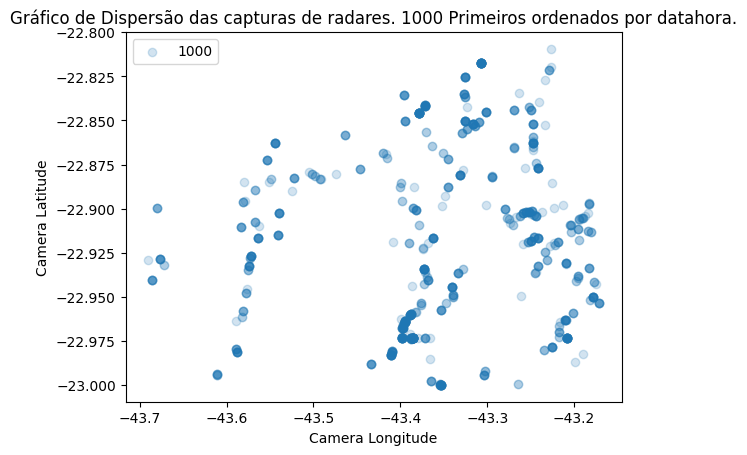
\includegraphics[width=0.7\linewidth]{disp1000.png}
\caption{\label{fig:disp1k} Gráfico de Dispersão das capturas de radares. 1000 Primeiras capturas ordenados por \textit{datahora}.}
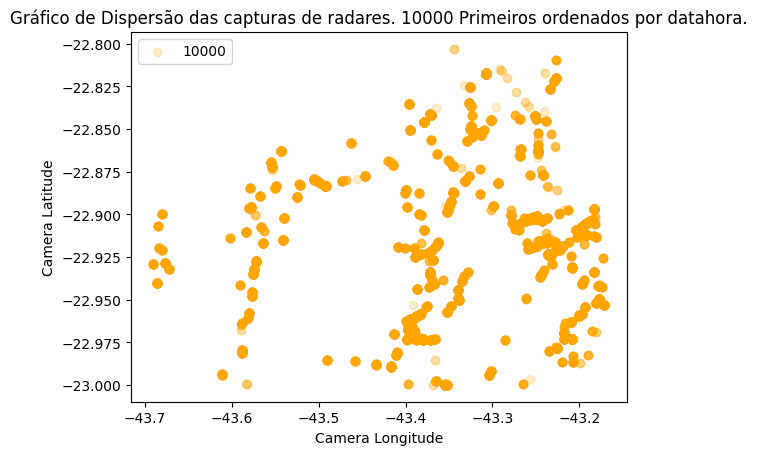
\includegraphics[width=0.7\linewidth]{disp10k.png}
\caption{\label{fig:disp10k} 10000 Primeiras capturas ordenados por data e hora.}
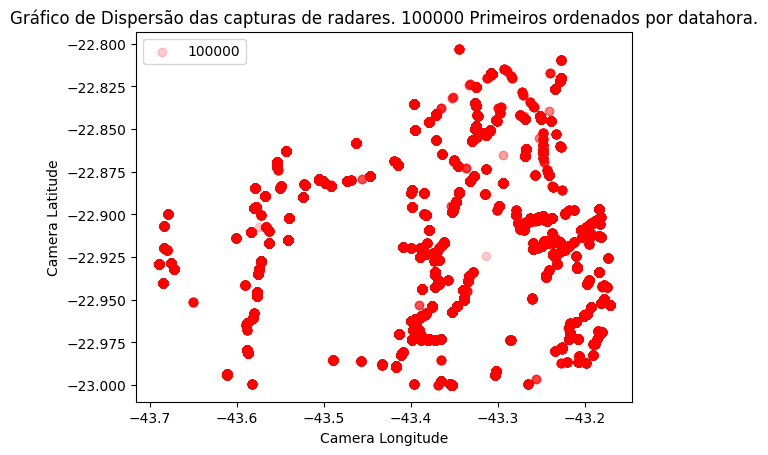
\includegraphics[width=0.8\linewidth]{disp100k.png}
\caption{\label{fig:disp100k} 100000 Primeiras capturas ordenados por data e hora. Podemos observar claramente a Zona Sul no canto inferior direito, a costa oeste da Baia de Guanabara, a Linha Amarela, a Barra na parte inferior, até a Estrada das Furnas/ Av. Édison Passos, cortando o Parque Nacional da Tijuca.}
\end{figure}

Sobrepondo alguns dos pontos em um mapa do município obtemos \ref{fig:disp1000Map}.

\begin{figure}
    \centering
    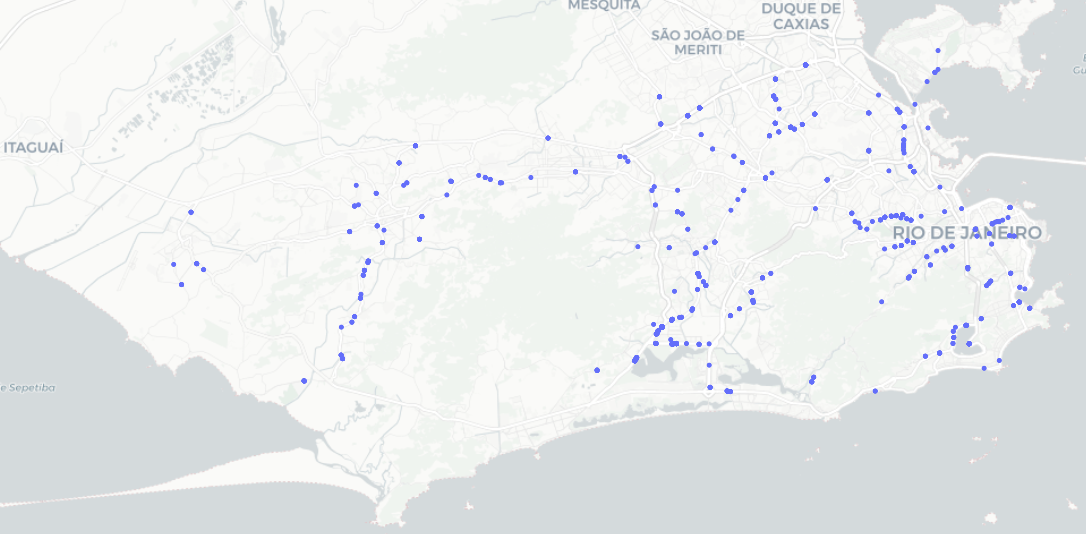
\includegraphics[width=1.0\linewidth]{disp1000Map2.png}
    \caption{Dados das primeiras 1000 detecções disponíveis da tabela, sobrepostos no mapa do Município do Rio de Janeiro.}
    \label{fig:disp1000Map}
\end{figure}

\section{Placas Clonadas}

\subsection{Mesma placa em dois veículos de tipos diferentes}

Uma maneira simples de detectar placas potencialmente clonadas é verificar se existem dois (ou mais) registros da mesma placa na tabela com valores de \textit{tipoveiculo} distintos. Isso indica que uma mesma placa está sendo utilizada em veículos distintos, ou, potencialmente, que houve algum erro no processo de detecção do \textit{tipoveiculo} no momento da captura. 

\begin{lstlisting}[language=SQL,caption={Query SQL para identificar inconsistências de placa com tipo de veículo. São retornadas todas as placas as quais existem dois (ou mais) registros na tabela com valores de \textit{tipoveiculo} distintos.},label={lst:sqlquery5}]
SELECT placa FROM `rj-cetrio.desafio.readings_2024_06`
GROUP BY placa HAVING COUNT(DISTINCT tipoveiculo) > 1;
\end{lstlisting}

Seguindo este critério, encontramos 441.652 placas inconsistentes.

Para identificar o segundo caso (erro na detecção do \textit{tipoveiculo}), podemos analisar os identificadores dos radares, verificando se existe algum padrão que indique falhas sistemáticas em um ou mais dos radares, o que geraria falsos positivos.



% Podemos então checar se é o caso previamente mencionado, onde uma (ou poucas) câmera(s) de radar possuí(em) erros sistemáticos de detecção do tipo de veículo.

\subsection{Distância entre dois registros}

Outra maneira de identificar placas clonadas é verificar a existência de dois registros da mesma placa, distantes um do outro, com uma pequena diferença de \textit{datahora\_captura}. Podemos assumir que, dada uma distância suficientemente grande e uma diferença entre \textit{datahora\_captura} ($\Delta t$) suficientemente pequena, é impossível que seja o mesmo veículo em ambos os locais.

\subsubsection{Distância em linha reta}

Dadas a latitude e longitude de dois registros, podemos calcular sua distância em kilômetros utilizando a fórmula de "haversine". Para melhor performance, calculamos diretamente na query SQL para apenas buscar os dados relevantes para análises subsequentes.

\begin{lstlisting}[language=SQL,caption={Fórmula de haversine para calcular distâncias em kilometros na superfície da Terra, através de latitudes e longitudes.},label={lst:sqlquery6}]
 6371 * ACOS(
      COS(RADIANS(t1.camera_latitude)) * COS(RADIANS(t2.camera_latitude)) *
      COS(RADIANS(t2.camera_longitude) - RADIANS(t1.camera_longitude)) +
      SIN(RADIANS(t1.camera_latitude)) * SIN(RADIANS(t2.camera_latitude))
    ) AS distance_km
\end{lstlisting}

\begin{lstlisting}[language=SQL,caption={Fórmula de haversine para calcular distâncias em kilometros na superfície da Terra, através de latitudes e longitudes. Sem acesso à função RADIANS() nem PI() e resolvendo erro de float point precision na função ACOS().},label={lst:sqlquery7}]
6371 * ACOS(LEAST(GREATEST(
      COS(t1.camera_latitude * 3.141592 / 180) * COS(t2.camera_latitude * 3.141592 / 180) * 
      COS(t2.camera_longitude * 3.141592 / 180 - t1.camera_longitude * 3.141592 / 180) + 
      SIN(t1.camera_latitude * 3.141592 / 180) * SIN(t2.camera_latitude * 3.141592 / 180),-1),1)) AS distance_km
\end{lstlisting}

Com essa função de distância, podemos observar alguns casos de mesma placa com registros de distâncias grandes, em um curto período de tempo.

\begin{lstlisting}[language=SQL,caption={Exemplo de query SQL para detectar inconsistências e retornar casos de mesma placa com registros distantes um do outro, segundo a fórmula de haversine, mas com diferença de tempo entre eles de curta. Considerando inconsistente percorrer mais de 6km em menos de 3 minutos (120km/h de média). Como discutido no artigo, podemos substituir última condicional WHERE para "time\_diff\_minutes $ \leq $ distance\_km/5" para melhor resultados.},label={lst:sqlquery8}]
WITH distance_time_check AS (
  SELECT
    t1.placa,
    t1.datahora AS datahora1,
    t2.datahora AS datahora2,
    t1.camera_latitude AS lat1,
    t1.camera_longitude AS lon1,
    t2.camera_latitude AS lat2,
    t2.camera_longitude AS lon2,
    ABS(TIMESTAMP_DIFF(t1.datahora, t2.datahora, MINUTE)) AS time_diff_minutes,
    6371 * ACOS(LEAST(GREATEST(
      COS(t1.camera_latitude * 3.141592 / 180) * COS(t2.camera_latitude * 3.141592 / 180) * 
      COS(t2.camera_longitude * 3.141592 / 180 - t1.camera_longitude * 3.141592 / 180) + 
      SIN(t1.camera_latitude * 3.141592 / 180) * SIN(t2.camera_latitude * 3.141592 / 180),-1),1)) AS distance_km
  FROM
    `rj-cetrio.desafio.readings_2024_06` t1
  JOIN
    `rj-cetrio.desafio.readings_2024_06` t2
  ON
    t1.placa = t2.placa
    AND t1.datahora < t2.datahora
  WHERE t1.camera_latitude < -22.8 AND t2.camera_latitude < -22.8 
  AND t1.camera_latitude > -23.0  AND t2.camera_latitude > -23.0 
  AND t1.camera_longitude > -43.8  AND t2.camera_longitude > -43.8
  AND t1.camera_longitude < -43.1  AND t2.camera_longitude < -43.1
)
SELECT
  placa,
  datahora1,
  datahora2,
  lat1,
  lon1,
  lat2,
  lon2,
  time_diff_minutes,
  distance_km
FROM
  distance_time_check
WHERE
  time_diff_minutes <= 3 -- Threshold para diff em minutos
  AND distance_km >= 6   -- Threshold para diff em kilometros
ORDER BY
  placa, datahora1;
\end{lstlisting}

\begin{longtable}{|l|l|l|l|l|l|l|}
\hline
TO\_HEX(placa)  & lat1 & long1 & lat2 & long2 & Distância (km) & $\Delta t$ (min)  \\ \hline
AAEd0Z1N8R0nW6PjvFdY3uE= & -22.949    & -43.177    & -22.903 & -43.245 & 8.68  & 2         \\ \hline
AAFHNUra1M70d1Cw4bhU5VU= & -22.954 & -43.193   & -22.817 & -43.307    & 19.22 & 0    \\ \hline
AAAHLRM713ANhx0EEbTttcx8= & -22.880 & -43.331   & -22.835 & -43.245  & 9.63 & 0    \\ \hline
AAHtSwsIG2PODaQXtXb9gQs= & -22.940 & -43.367   & -22.994 & -43.303   & 8.89 & 2   \\ \hline
AAJbkMjCdI3+qr77FZOTSRo= & -22.936 & -43.333   & 22.979 & -43.588  & 26.58 & 3  \\ \hline
\caption{\label{tab:results1}  Tabela com alguns dos dados de retorno do SQL \ref{lst:sqlquery8}. É impossível que um mesmo veículo percorra distâncias como 26,6km em 3 minutos, ou até 19,2 km em 0 minuto. Logo são casos claros de falha nos radares e/ou placas clonadas.}
\end{longtable}

Utilizando tal abordagem, com limites de "\textit{time\_diff\_minutes} $\leq 3 $ E \textit{distance\_km} $ \geq 6$", conseguimos detectar 104142 casos de placas distintas com indícios de clonagem.

Podemos deixar mais genérica a condição de inconsistência, já que podem existir casos de registros que percorrem, por exemplo, 8km em 4min, a mesma velocidade inconsistente, porém a SQL atual não os mostra. Para detectar todos os casos onde a distância e o $\Delta t$ são potencialmente inconsistentes, podemos utilizar a condicional "\textit{time\_diff\_minutes} $\leq$ \textit{distance\_km}/2". Assim capturamos todos os casos que acarretariam uma velocidade média de mais de 120km/h, num total de 636811 placas distintas suspeitas. Esse número elevado pode apontar um número significativo de falsos positivos.

Para garantir um número menor de falsos positivos, já que numa via expressa é possível alguns veículos alcaçarem tal velocidade, utilizaremos "\textit{time\_diff\_minutes} $\leq$ \textit{distance\_km}/3", necessitando de 180km/h de média para percorrer a distância entre registros no tempo indicado. Utilizando tal condicional temos um resultado final de 621552 casos distintos de placas com registros inconsistentes.

Para finalizar, e garantir nenhum falso positivo, podemos utilizar uma condicional mais extrema como \textbf{"\textit{time\_diff\_minutes} $ \leq $ \textit{distance\_km}/5"}, só possível se o veículo mantivesse \textbf{300km/h}, numa linha reta entre os dois ponto, já que não é possível, identificamos então \textbf{610606 casos de placas clonadas} utilizando este critério.

\subsubsection{Distância no trânsito}

Para uma estimativa mais precisa do tempo esperado para percorrer uma distância entre dois pontos, o ideal seria considerar, ao invés de uma linha reta, a geografia e o urbanismo da Cidade. Identificando o endereço referente ao ponto geolocalizado (por latitude e longitude) e então utilizar bilbliotecas de estimativa de tempo mínimo no trânsito para percorrer a distância entre os dois registros. Assumir que se uma placa foi registrada nesses dois pontos em um tempo significativamente menor que tal estimativa, um erro de registro ou placa clonada existe.

Tal abordagem seria claramente mais custosa, porém como os registros são fixos nos radares, e temos apenas 1421 radares únicos, podemos calcular a distância par-a-par entre os radares (2017820 valores), que podem ser utilizados para estimar o $\Delta t$ mínimo para todos os pares de registros de cada \textit{placa}.

Para uma precisão ainda melhor, podemos utilizar a datahora de captura e os dados de trânsito do momento da caputura, porém não poderíamos mais aproveitar do agrupamento dos mais de 30 milhões de valores nos 1421 radares, requerendo novamente executar um chamado a biblioteca de estimativa de tempo no trânsito para cada par de registros suspeitos, o que poderia ser computacionalmente inviável.

\subsection{Placas Falsas}

Também é interessante considerar a possibilidade da criação ilegal de placas não registradas. Tal evento não se caracterizaria como uma clonagem, porém com acesso aos números e letras da placa é viável a realização de uma checagem simples se tal placa é realmente válida. Esta verificação poderia se dar através de uma requisição à um sistema conectado ao cadastro geral.

\section{Ferramentas utilizadas}

Para o desenvolvimento da análise documentada neste artigo, foram utilizadas as seguintes ferramentas:

\begin{enumerate}
\item Google BigQuery para acesso à tabela "rj-cetrio.desafio.readings\_2024\_06", execução de queries SQL, e execução de notebook Python conectado à tabela,
\item Python e Bibliotecas de análise de dados - pandas para analisar DataFrames com grande quantidade de dados, matplotlib e plotly para análises gráficas,
\item Overleaf - Editor LaTeX, para documentar algumas das SQL usadas e tabelar valores, além de facilitar a organização e apresentação do trabalho,
\item Excalidraw, para organização de ideias relativas ao desafio (Figura \ref{fig:excalidraw}).
\end{enumerate}

\begin{figure}
    \centering
    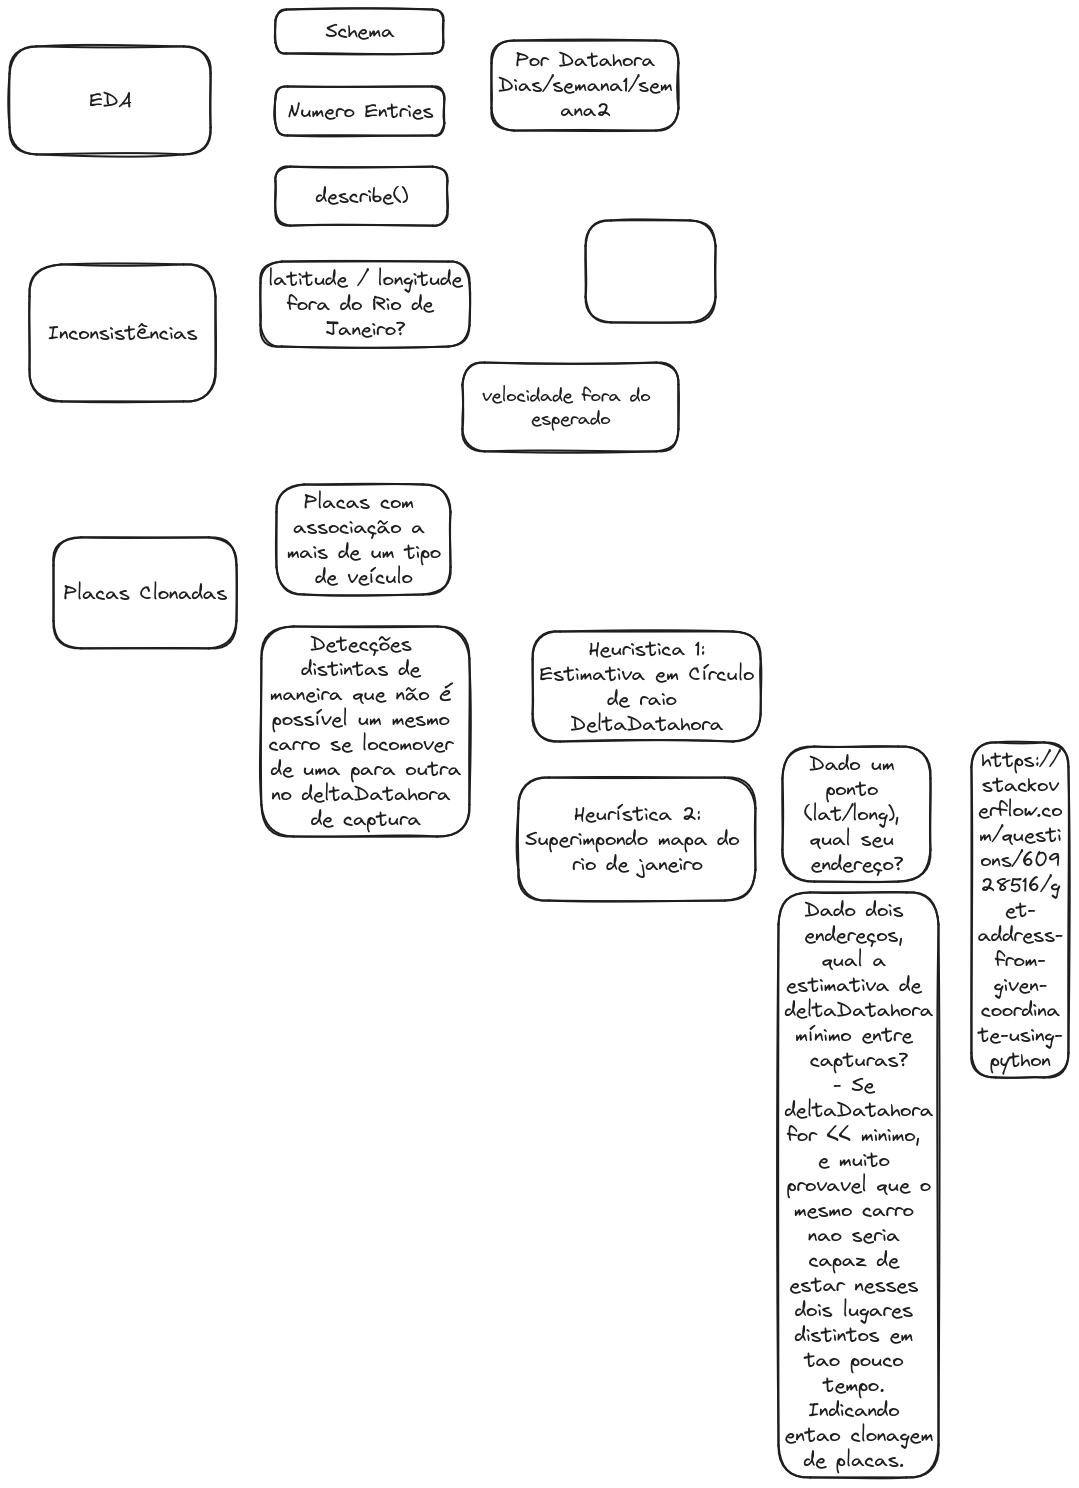
\includegraphics[width=0.9\linewidth]{excalidraw.png}
    \caption{Artefato da ferramenta Excalidraw, utilizado na organização prévia e durante o desenvolvimento deste artigo.}
    \label{fig:excalidraw}
\end{figure}

\section{Próximos Passos}

Nesta análise assumimos uma série de simplificações, tais como:
\begin{enumerate}
\item Desconsiderar totalmente valores de latitude/longitude fora de um modelo retângular do Rio de Janeiro.
\item Distância em linha reta entre pontos geolocalizados para estimativa $ \Delta t $ mínimo,
\item Considerar todas as câmera de radares que registram latitudes e longitudes corretas como confiáveis.
\end{enumerate}


Como proximos passos, para refinar os resultados, poderíamos:
\begin{enumerate}
\item Verificar a possibilidade de corrigir valores de latitude/longitude inconsistentes: Por exemplo, obter de fonte confiável os valores de cada um dos 1421 radares, desta forma obtendo ~20\% mais registros para análise.
\item Obter uma distância entre dois registros seguindo as ruas e tempos históricos de trânsito no Município: Por exemplo, uma função que retorne o endereço dada sua latitude e longitude, e outra função que recebe dois endereços e retorna o tempo esperado utilizando bibliotecas (ex. google.maps.MapsLibrary) externas.
\item Analisar a possibilidade de uma ou poucas câmeras de radar estarem gerando dados errados, com placas ou tipo de veículo mal identificados, ou com datahora e/ou latitude/longitude equivocadas. Se identificados radares com tais problemas, remover os registros associados à ele do dataset. Assim diminuiríamos significativamente a quantidade de falsos positivos na solução proposta.
\end{enumerate}


\end{document}